\documentclass[12pt]{article}
\usepackage[utf8]{inputenc}
\usepackage[T5]{fontenc}
\usepackage{graphicx,a4wide,framed,amsmath}

\newcommand{\source}[1]{\begin{flushright}\emph{[#1]}\end{flushright}}

\newcommand{\MakeScribeTop}[1]{
\noindent
\begin{framed}
\noindent
 Algorithmique Avancée 2019
 \hfill
 École Centrale-Supélec
 \\[1em]
 \centerline{ \Large
#1
 }
 \\[1em]
\centerline{  \it Christoph Dürr, Nguyễn Kim Thắng}
\end{framed}
}



\begin{document}
    \MakeScribeTop{Corrections}

\section{Diviser pour régner et algorithme glouton}

\subsection{Cartes bancaires}

    L'instance est un ensemble de points $G=\{1,\ldots,n\}$. Il est partionné
en classes d'équivalence, mais ce partionnement n'est pas donné. Il faut le
découvrir par des tests sur des paires de points. Une classe est géante si sa
taille fait au moins la moitié de $G$.

On pourrait être tenté de calculer le partionnement de $G$ en classes d'équivalence.
Nous décrivons ici cette approche puis observons les problèmes.  
Pour un algorithme par diviser et régner, le cas de base est $|G|\leq 1$, et il est trivial.

Si $|G|\geq2$ on commence par partager $G$ arbitrairement en deux parties,
$A,B$ avec  $|A|=\lfloor n/2 \rfloor, |B|=\lceil n/2 \rceil$. On calcule
récursivement les partionnements ${\cal P}_A,{\cal P}_B$ de respectivement $A$
et $B$.  Puis pour trouver le partitionnement $\cal P$ de $G$, on doit juste
découvrir quelles sont les paires de parties de ${\cal P}_A$ et de ${\cal P}_B$
dont l'union forme une partie de $\cal P$.  Le problème est que cette
opération prendra un temps de l'ordre de $|{\cal P}_A| \cdot |{\cal P}_B|$
dans le pire des cas, ce qui peut être quadratique.

La clé est de calculer seulement les classes géantes du partionnement.  En
effet, si $C$ est une classe géante de $G$, alors soit $C\cap A$ est géante
pour $A$ soit $C\cap B$ est géante pour $B$ ou les deux à la fois.   Soit
$f(G)$ l'ensemble des classes géantes de $G$. Cet ensemble contient 0, 1 ou 2
classes. Chaque classe est identifié par sa taille et de ses éléments, qui
peut être arbitraire. Donc si à la fois $f(A)$ et $f(B)$ sont vides, on peut
répondre $f(G)=\emptyset$ également. Sinon on doit pour chaque partie géante
de $f(A)\cup f(B)$, vérifier si elle se complète en une classe géante dans
$G$.  Pour chaque partie géante dans $A$, il faut faire des tests avec tous
les éléments dans $B$, donc $n/2$ tests au plus. Comme $|f(A)\cup f(B)|\leq
4$, ceci représente au plus $2n$ tests par appel récursif.

     \centerline{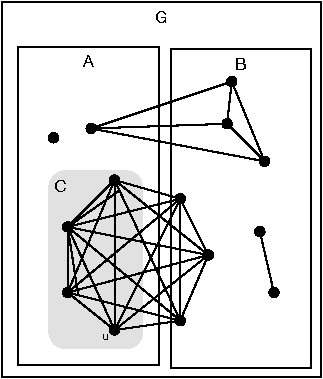
\includegraphics{grande_clique.pdf}}

     Pour l'analyse de la complexité, on note $T(n)$ une majoration sur le
     temps passé par l'algorithme pour un graphe de taille $n$.  On a $T(0) =
     T(1) = 0$, ainsi que $T(n) \leq 2n + T(\lceil n/2 \rceil)+ T(\lfloor n/2
     \rfloor) \leq 4n \log n$. Pour s'en convaincre, remplacez $n$ par la
     prochaine puissance de $2$, disons $n'$, ceci ne pourra que augmenter la
     complexité et $n$ n'augmentera que d'un facteur au plus $2$.  Comme il y
     a exactement $\log_2 n'$ appels récursifs, on obtient la complexité
     annoncée.

\subsection{Placement d'antennes}


\paragraph{Observation}
Quand on trace un cercle autour de chaque île de rayon $r$, on découvre un intervalle sur la plage qui doit contenir une antenne. Le problème se réduit alors au problème suivant.

\paragraph{Ensemble minimum de points intersectant chacun des intervalles donnés}
Pour $n$ intervalles donnés $[a_1,b_1],\ldots,[a_n,b_n]$, il faut trouver un ensemble de points $S$ de cardinalité minimale tel que chaque intervalle intersecte $S$.

\paragraph{Algorithme glouton par balayage en $O(n\log n)$.} 

On traite tous les intervalles dans l'ordre croissant de leur côté droit. 
Désormais on suppose $b_1\leq \ldots\leq b_n$. Ce tri coûte un temps $O(n \log
n)$ est constitue le goulot d'étranglement. La suite ne prend qu'un temps
linéaire.

À tout moment on maintient une solution $S$ pour les intervalles déjà vus, qui
minimise $|S|$ et en cas d'égalité maximise $\max S$.

L'algorithme est simple.  On débute par $S=\emptyset$ et pour tout
$i=1,\ldots,n$, si on a $a_i\leq max S$, alors on ne fait rien, sinon on
ajoute $b_i$ à $S$. L'idée est qu'il faut de toute façon couvrir $[a_i,b_i]$
et en choisissant la valeur la plus grande qui le couvre, on augmente la
chance de couvrir également les intervalles traités par la suite.

Formellement, soit $I_x$ l'ensemble des intervalles $[a_j,b_j]$ avec $x<a_j$
et $f_x$ la solution optimale pour $I_x$. Comme $I_x \supseteq I_y$ pour tout
$y\geq x$, on a que $f_x$ est monontone décroissant en $x$ (pas strict).  Si
$I_x$ est vide, alors $f_x=0$. Sinon $f_x=1+\min_{y\in[a_j,b_j]} f_y$, où
$[a_j,b_j]$ est un intervalle de $I_x$ qui minimise $b_j$. Par monotonocité de
$f$, le choix $y=b_j$ est optimal.

\subsection{Gestion de cache}

Cette question est peut-être parmi les plus difficiles.  Il faut donner un
argument d'échange pour montrer qu'on peut transformer toute solution $S$ en
une qui suit la politique FF.  Le problème est que si on modifie un
remplacement dans $S$, ceci a un effet sur toute la suite.  Il faut donc faire
une autre transformation sur $S$ plus tard pour resynchroniser les caches dans
les deux solutions.  Pour une explication complète nous vous renvoyons à la
section 4.3 "Optimal Caching: A more complex exchange argument" du livre
"Algorithm design" de Jon Kleinberg et Éva Tardos.


\section{Programmation dynamique 1}

\subsection{Arbre binaire de recherche optimal}

Contre-exemples: Si on prend à chaque fois l'élément de plus grande fréquence
comme racine, on aura une solution non optimale pour $f_i=1+i \epsilon$ avec
$\epsilon >0$ arbitrairement petit. Si on prend à chaque fois l'élément qui
équilibre les fréquences à gauche et à droite on, on aura une solution non
optimale pour $f=(1,0,1)$.


Soit $A[i,k]$ le coût de l'arbre de recherche optimal pour le problème
restreint aux éléments de $i$ à $k$. Notons $T[i,k]$ cet arbre.

  Les cas de base sont $A[i,i]=f_i$ et $A[i,i-1]=0$ pour l'arbre vide. (On pourrait se restreindre aux cas de base $k=i-1$, mais pour plus de lisibilité on inclu $k=i$.) 
Pour $i<k$, l'arbre optimal a bien une racine, disons avec l'élément $j$ pour $i\leq j\leq k$.  

Observation clé: Le sous-arbre gauche est un arbre optimal pour les élements de $i$ à $k-1$, car si on pouvait le remplacer par un arbre meilleur ceci diminuerait également le coût de $T[i,k]$ et contredirait son optimalité.  Il en est de même pour le sous-arbre droit.

Donc $T[i,k]$ a la forme $\textrm{tree}(T[i,j-1],j,T[j+1,j])$ pour un certain $k$, et où tree dénote le constructeur d'un arbre binaire. Quel est le coût de l'arbre~?
Les éléments du sous-arbre gauche ont une profondeur plus grande de $1$ dans $T[i,k]$ que dans $T[i,j-1]$. Il faut donc ajouter $f_i + \ldots +f_{j-1}$ au coût de $T[i,j-1]$, qui par définition est $A[i,j-1]$.  On a la même situation avec sous-arbre droit. Et la racine génère un coût de $f_j$.  Ces observation mènent vers la récursion pour $i \leq k$
\[
	A[i,k] = f_i + \ldots + f_k +  \min_{i\leq j\leq k} (A[i,j-1] + A[j+1,j]).
\]


     \centerline{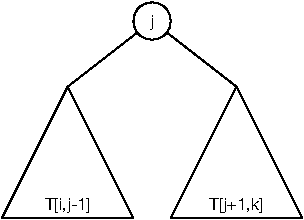
\includegraphics{arbre_bin_rech_opt.pdf}}


On a $O(n^2)$ variables à calculer, chacune est une minimisation sur $O(n)$ alternatives. Au total la complexité est de $O(n^3)$.
Ces variables doivent être calculées dans un bon ordre. Une possibilité est de boucler sur toutes les valeurs $k=1,2,\ldots, n$ et à l'intérieur de boucler sur toutes les valeurs $i=k,k-1, k-2, \ldots, 1$ dans cet ordre.

Pour calculer l'arbre proprement dit il suffit de stocker dans une matrice auxiliaire $B$, la valeur $B[i,k]=j$ où $j$ est le minimiseur de la récursion pour $A[i,k]$.  Ensuite la fonction récursive \textsl{build\_tree}$(i,k)$ va retourner l'arbre vide si $k<i$ et sinon retournera 
\[
\textrm{tree}(\textsl{build\_tree}(i,B[i,k]-1), B[i,k], \textsl{build\_tree}(B[i,k]+1,n)).
\]
Cette construction aura une complexité linéaire en $n$ car un travail constant est effectué pour chaque nœud.


\subsection{Distance d'édition}

Similaire à la plus longue sous-séquence commune.
Sous-problème défini par les préfixes $x_1,\ldots,x_i$ et $y_1,\ldots,y_j$.
Soit $A[i,j]$ la distance d'édition entre ces préfixes. 
Cas de base: $A[0,j]=j$ insertions et $A[i,0]=i$ suppressions.
Si $x_i=y_j$, alors il existe une solution optimale qui ne touche pas à ces deux lettres et $A[i,j]= A[i-1,j-1]$ dans ce cas.

\begin{quote} Pour s'en convaincre considérons les paires de lettres
$(x_a,y_b)$ qui sont des lettres à n'avoir subi aucune opération d'édition, et
tel que $x_a$ est devenue la lettre $y_b$ dans $y$.  Appelons ces paires, les
\emph{paires correspondantes}.  Ces paires correspondantes sont sans
croisements, dans le sens si $(x_a,y_b)$ est une paire ainsi que
$(x_{a'},y_{b'})$ et $a<a'$ alors $b<b'$.  Alors minimiser le nombre
d'opérations d'édition, revient à maximiser le nombre de paires
correspondantes sans croisement.  Supposons $x_i=y_j$, et supposons que dans
la solution optimale $(x_i,y_j)$ n'est pas une paire correspondante. Alors une
des lettres, disons $x_j$ est forcément déjà mise en correspondance avec une autre
lettre disons $y_k$ pour $k<j$.  En remplaçant cette correspondance par
$(x_i,y_j)$, on ne crée pas de croisement, et on n'altère pas le nombre de
paires.  On a donc obtenu une solution avec la propriété demandée. \end{quote}

Sinon, si $x_i\neq y_j$, forcément au moins une des lettres $x_i,x_j$ a subi une des trois opérations, et donc dans ce cas
\[
A[i,j] = 1 + \min\{ \underbrace{A[ i,j-1 ]}_{\textrm{insertion $y_j$}}, 
 \underbrace{A[i-1,j]}_{\textrm{suppression $x_i$}}, 
 \underbrace{A[i-1,j-1]}_{\textrm{substitution $x_i \rightarrow y_j$}} \}.
\]

\subsection{Corriger un mot bien parenthésé}

D'abord on peut observer qu'il suffit de supprimer des parenthèses pour
corriger un mot. Une insertion n'a de but que de coupler une parenthèse isolé,
qu'on aurait pu supprimer.

Soit $x$ le mot d'entrée de longueur $n$, avec les indices allant de $0$ à $n-1$.
Notons $A[i,j]$ le plus petit nombre de suppressions nécessaires pour corriger le mot $x_i\ldots x_j$.  
Si $j<i$, on a $A[i,j]=0$ pour le mot vide.

Sinon, si $x_i=)$, alors $A[i,j]=1+A[i+1,j]$ clairement.
Maintenant considérons le cas $x_i=($.  Soit on supprime cette lettre, soit on l'associe avec une autre lettre $x_k=)$, avec $i<k\leq j$. D'où la récursion
\[
A[i,j] = 
\left\{
    \begin{array}{ll}
    1 + A[i+1,j] & \textrm{si } x_i=\textrm{)}
    \\
    \min\{1+A[i+1,j], \min_{i<k\leq j:x_k=)} A[i+1,k-1]+A[k+1,j]\} & \textrm{si } x_i=\textrm{(}.
    \end{array}
\right.
\]

Cependant il existe un algorithme glouton pour ce problème, de complexité
$O(n)$.  L'optimalité
vient du fait qu'il n'y ait pas vraiement de choix quand au jumélage des
parenthèses. On balaye la chaîne de gauche à droite.  On partitionne la partie
déjà traitée en trois parties. Des paires de parenthèses ouvrante-fermante. Des
parenthèses ouvrantes qui n'ont pas encore vu leur pendant. Et des parenthèses
fermantes qui doivent être supprimées, car elles n'ont pas de pendant ouvrant.

Pour cela, on maintient un compteur de profondeur $p$. Et on stocke dans un
tableau $t[k]$ l'indice de la dernière parenthèse ouvrante de profondeur $k$
rencontrée, qui n'a pas encore eu son pendant de parenthèse fermante.

Initialement $p=0$. Pour tout $i=1,\ldots,n$, si $x_i$ est une parenthèse
ouvrante, alors on stocke $t[p]=i$ et on incrémente $p$.  Notez que $t[p]$
était forcément indéfini.

Si $x_i$ est une parenthèse fermante, alors on décrémente $p$.  Si $p<0$ ou
$t[p]$ n'est pas défini, alors on doit supprimer $x_i$. Dans ce cas on annule
la décrémentation de $p$.  Dans le cas contraire on jumèle $x_i$ avec
$x_{t[p]}$ et on marque $t[p]$ comme indéfini pour la suite.

Après le traitement on se doit de supprimer toutes les parenthèses ouvrantes
de la forme $x_{t[k]}$ pour les entrées définis dans $t$.

\subsection{Parenthéser une expression booléenne}

Notons $C_0,\ldots, C_{n-1}$ les constantes et $O_{0},\ldots,O_{n-2}$ les
operateurs. Notons $A[i,j]$ le nombre de manières de placer des parenthèses
pour que l'expression $C_i O_i \ldots C_j$ soit vraie.

Notons $B[i,j]$ le nombre de placements de parenthèses qui rend l'expression fausse. 

Pour le cas de base $A[i,i]$ est la valeur de $C_i$, (1 pour T et 0 pour F).
Et $B[i,i]=1-A[i,i]$.

Pour $j>i$, on les récusions suivantes.
Pour un parenthèsage, la dernière opération est $O_k$ pour un indice $i\leq k < j$.
Cette dernière opération décompose l'expression en deux parties. Donc
$A[i,j]$ est la somme sur $k=i,\ldots,j-1$ de
\begin{align*}
    A[i,k]\cdot A[k+1,j] & \textrm{ si } C_k=\wedge \\
    A[i,k]\cdot A[k+1,j] + B[i,k]\cdot A[k+1,j] + A[i,k]\cdot B[k+1,j] & \textrm{ si } C_k=\vee \\
    B[i,k]\cdot A[k+1,j] + A[i,k]\cdot B[k+1,j] & \textrm{ si } C_k=\oplus.
\end{align*}
$B[i,j]$ peut être obtenu de manière similaire, c'est la somme sur $k=i,\ldots,j-1$ de
\begin{align*}
    B[i,k]\cdot B[k+1,j] + B[i,k]\cdot A[k+1,j] + A[i,k]\cdot B[k+1,j] & \textrm{ si } C_k=\wedge \\
    B[i,k]\cdot B[k+1,j] & \textrm{ si } C_k=\vee \\
    A[i,k]\cdot A[k+1,j] + B[i,k]\cdot B[k+1,j] & \textrm{ si } C_k=\oplus.
\end{align*}

\subsection{Rendu de monnaie}

\begin{itemize}
    \item Soient les pièces 1,4,5 et la valeur cible 8. Glouton produira 5+1+1+1 alors que l'optimum est 4+4.
    \item Chaque chiffre de l'écriture décimale de $R$ est un sousproblème indépendant.  En analysant les 10 cas, on prouve l'affirmation.
    \item
    Déterminer le nombre minimal de billets: 
    Soit $A[i,z]$ la solution optimale pour les pièces $x_0,x_1,\ldots,x_i$ et valeur cible $0\leq z\leq R$.
    Par convention $A[-1,z]=\infty$ et $A[i,z]=\infty$ pour $z<0$.
    Alors $A[0,0]=0$ et en géneral $A[i,z]=\min\{A[i-1,z],1+A[i,z-x_i]\}$.  

    La solution optimale est $A[n,R]$, il y a $O(nR)$ variables, chacune étant l'optimum sur deux options. 
\end{itemize}

\subsection{Partage équitable}

Notons $W=\sum w_i$.  Pour $0\leq v \leq W$ et $0 \leq i \leq n$, soit $T[i,v]$ un booléen qui indique s'il existe un ensemble $S\subseteq \{1, \ldots, i\}$ avec $\sum_{j\in S} w_j = v$.

Les cas de base sont $T[0,0]=$Vrai et $T[0,v]=$Faux pour tout $v>0$.
Sinon pour $i \leq 1$ et $v$ fixé l'ensemble de somme $v$ soit contient $i$ soit ne contient pas $i$.  Ceci donne la récursion suivante
\[
		T[i,v] = T[i-1, v] \vee T[i-1, v - w_i],
\]
où la dernière option n'est valable que si $v \geq w_i$.

Enfin le partage équitable peut être obtenu en cherchant la valeur $v$ la plus proche de $\sum w_i /2$ pour laquelle on ait $T[n,v]$.  Pour obtenir l'ensemble proprement dit, il faut maintenir dans un tableau auxiliaire lequel des deux choix de la récursion ci-dessous a rendu $T[i,v]$ vrai. Ceci permet de dérouler dans l'ordre décroissant des indices $i$, les éléments de l'ensemble $S$ de la solution.

\end{document}